\section{Discussion and Implications}
We do not use the image and the metadata in this project. We think the image and the metadata are important for the adoption speed. However, we do not have enough time to do the image analysis and the metadata analysis. We think the image analysis is a good direction for future research. Also, there is also a lot of information in the description of the pet. We think the description is also a good direction for future research. Though we don't use the image and the metadata, we think the result is good enough. A $\kappa$ of $0.4694$ is not bad since we only use 176 features to predict the adoption speed. 
\begin{figure}[H]
    \centering
    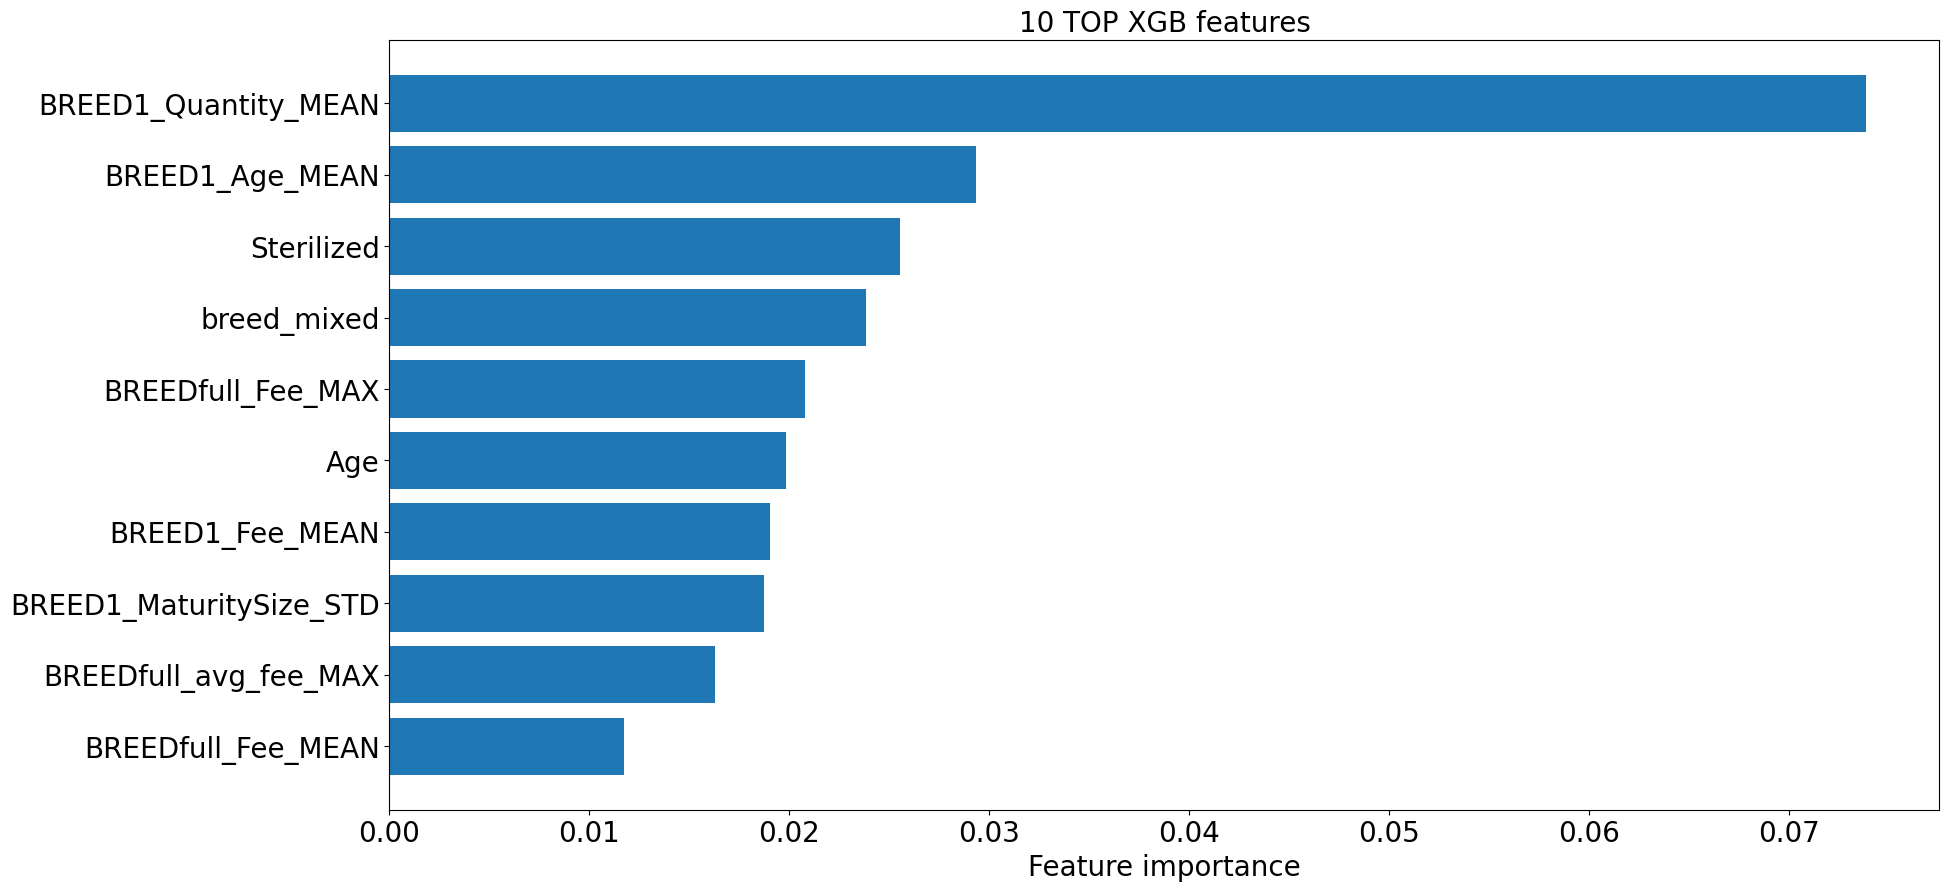
\includegraphics[width=1\textwidth]{code/figure/xgb_feature_importance.png}
    \caption{Feature importance}
    \label{fig:feature_importance}
\end{figure}
From \Cref{fig:feature_importance} we can see that, the main breed, i.e., Breed1, is the most important factor affecting the adoption speed. Also, whether is sterilized, whether is breed is mixed and the age of the pets are also important factors. This is intuitive since in reality, people tend to adopt pets with a younger age. Also, the sterilized status is also important since people tend to adopt pets that are sterilized. The color of the pet is not important. This is reasonable since the color of the pet is not a good indicator of the adoption speed. We can also see that, the adoption fee also matters. 

Thus, to improve the adoption speed, we can do the following things:
\begin{itemize}
    \item Highlight the main breed of the pet.
    \item Show mixed breed.
    \item Sterilize the pet.
    \item Highlight the age of the pet.
    \item Set a reasonable adoption fee.
\end{itemize}